\identify{Identify the Challenge \& Set Goals:  Intake V1.1 (July 25th, 2024)}
\chapterauthor{Caleb Bachmeier}
\info{Caleb Bachmeier}{Identify the Challenge \& Set Goals:  Intake Redesign}{July 25, 2024}
\textbf{Goal}: We will identify an objective for our robot so that we can address it and build an effective solution
\section*{Problem Statement}
We have discovered a problem in our intake design; when we are spinning our intake, the flaps get caught on the fifth ring we score. This stops out intakes movement, which also means we can't score a sixth ring. We before though this was a problem with our clamp, but know we know the real problem. This problem is shown in \blueref{intake-problem}{this figure.} 
\section*{Solution Requirements}
\begin{itemize}
    \item Must use VRC official parts
    \item Must not change our intake design too much
\end{itemize}
\section*{Solution Goals}
\begin{itemize}
    \item We need to find a efficient solution fast, before our deadline for finishing our first robot is over.
\end{itemize}
\begin{figure}[h!]
    \centering
    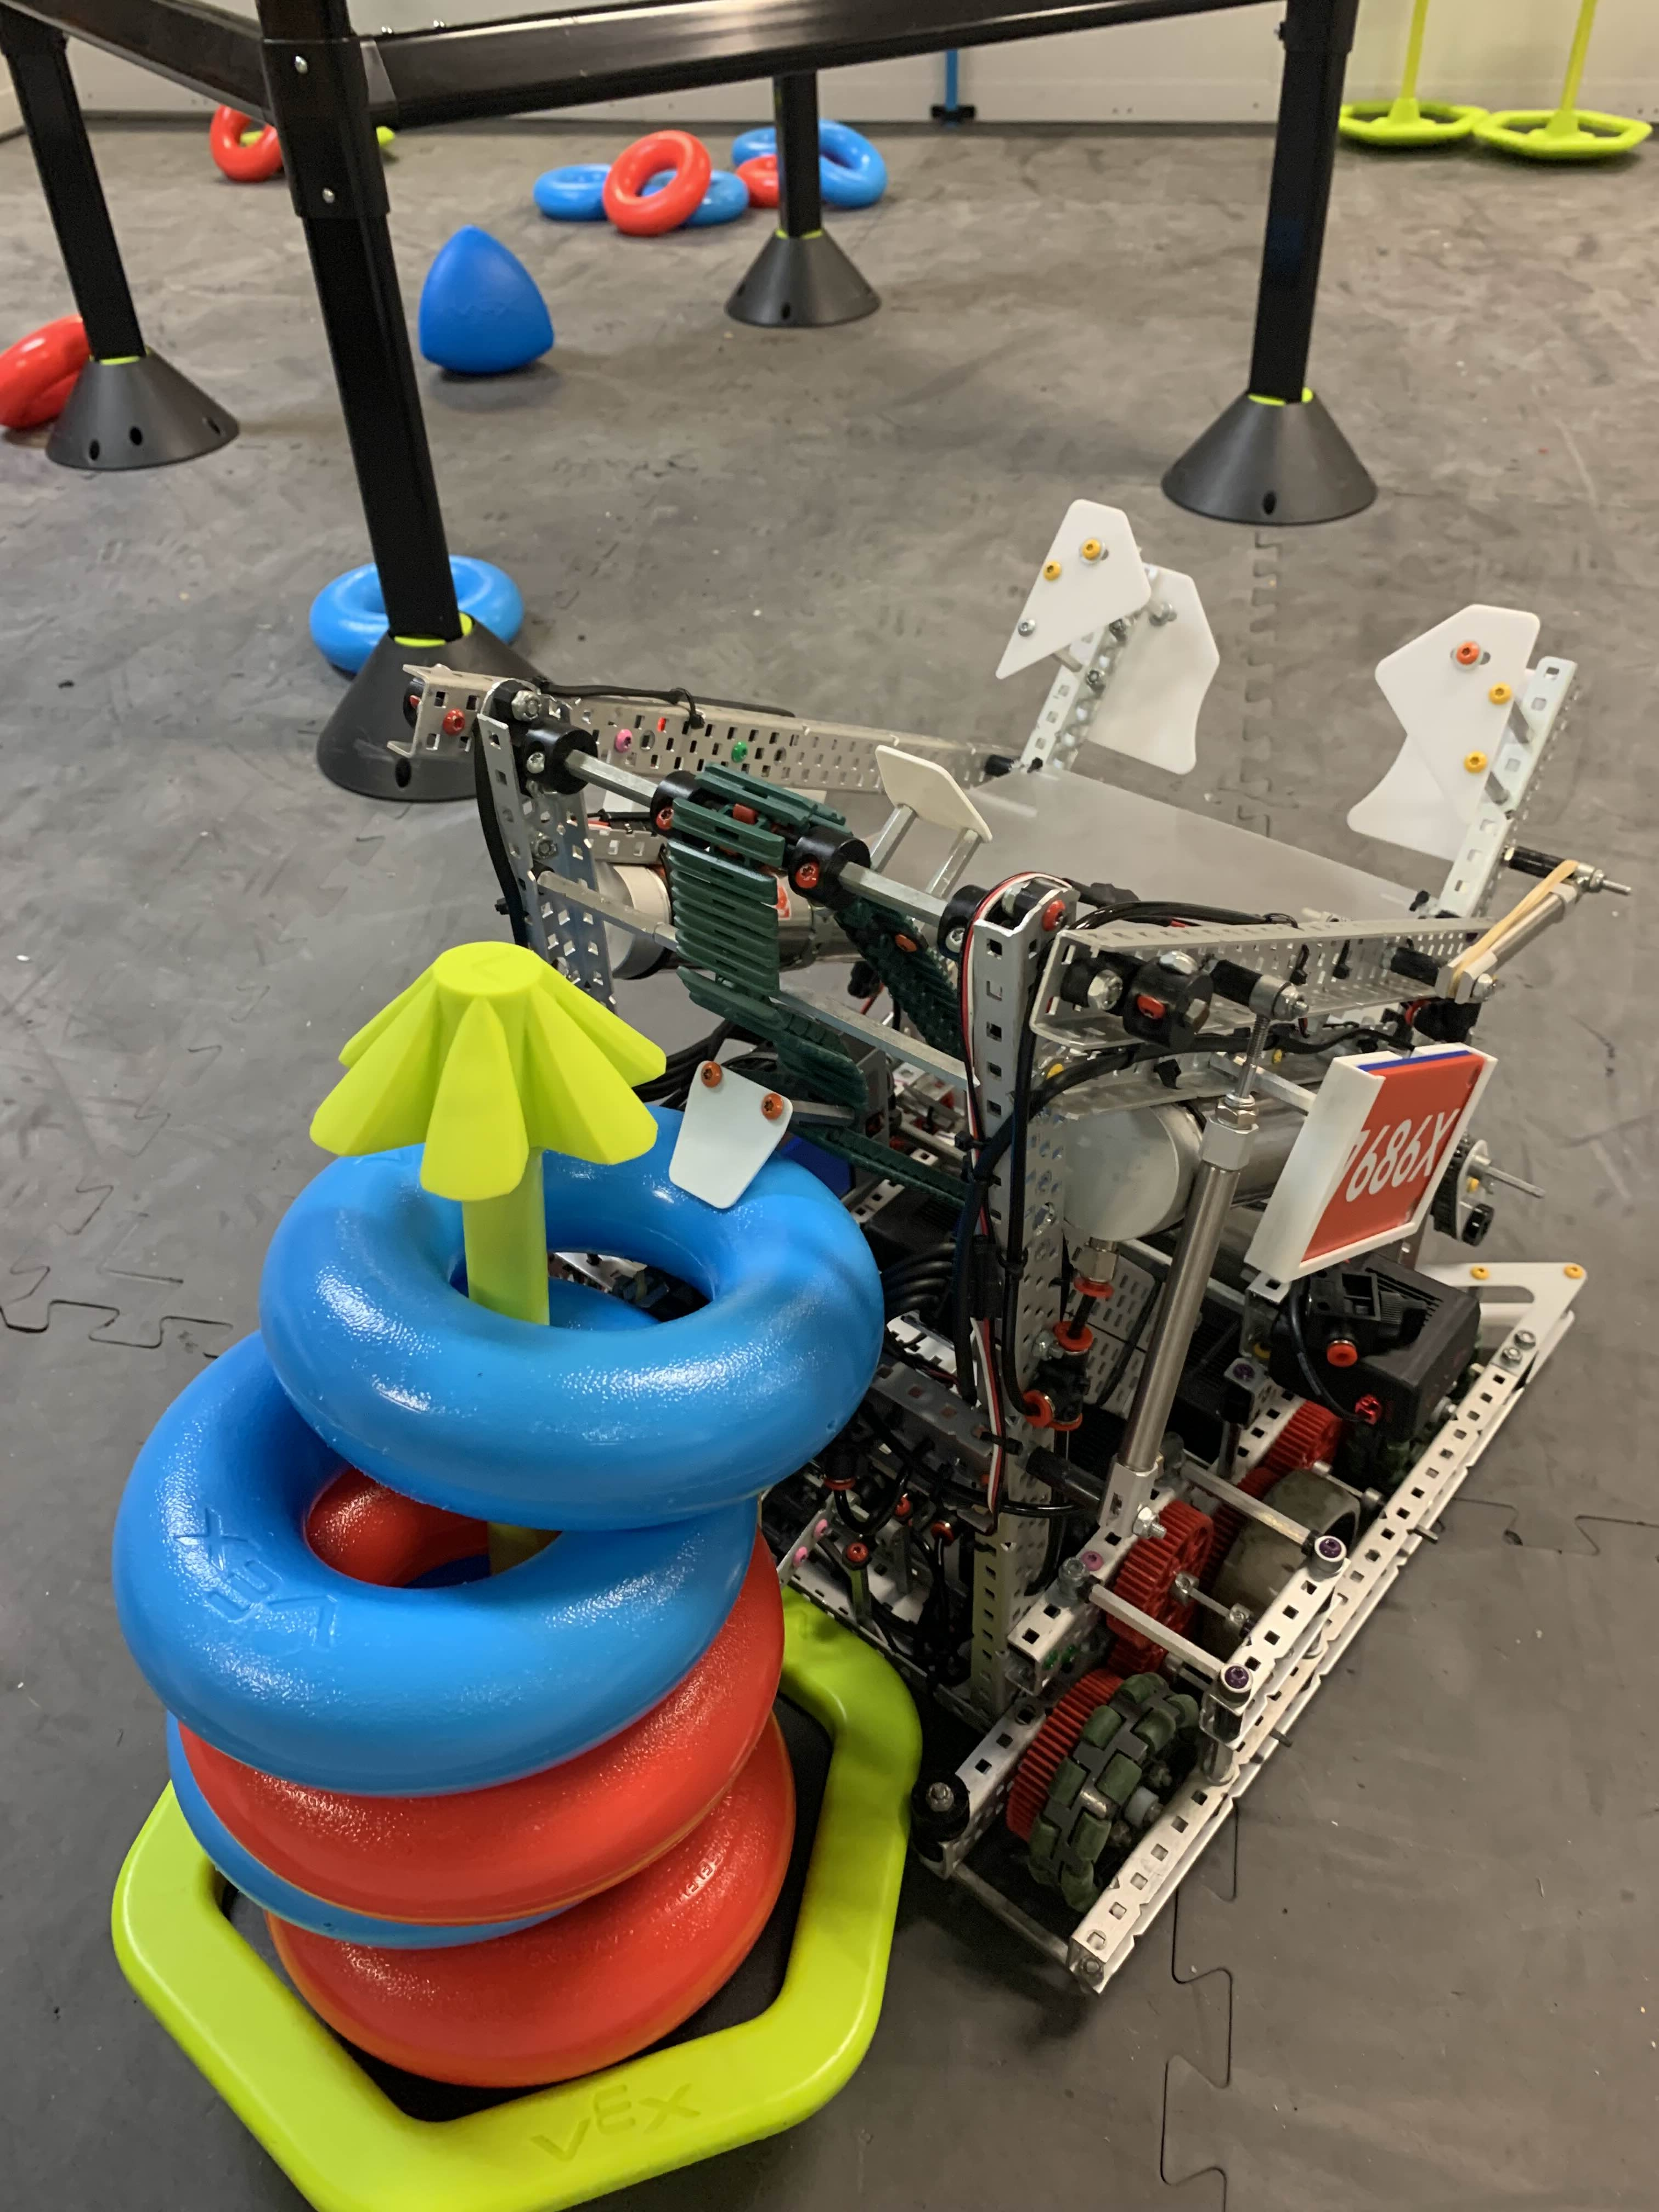
\includegraphics[width=0.5\linewidth]{images/Intake-problem.jpg}
    \caption{Our intake problem}
    \label{intake-problem}
\end{figure}
\brainstorm{Brainstorm \& Diagram: Intake V1.1 (July 25th, 2024)}
\chapterauthor{Caleb Bachmeier}
\info{Caleb Bachmeier}{Brainstorm \& Diagram}{July 25, 2024}
\section*{Possible Solutions}
\noindent
\textbf{Guard}

A guard would push the fifth ring up, allow the intake to spin, and allow us to score six rings on a mobile goal. 

\noindent
\textbf{Pros}:
\begin{itemize}
    \item Would be very easy to construct
    \item Would absolutely work
\end{itemize}
\textbf{Cons}:
\begin{itemize}
    \item Could get in the way of the intake
\end{itemize}

\noindent
\textbf{Pneumatic}

We could use pneumatic to push the fifth ring in place

\noindent
\textbf{Pros}:
\begin{itemize}
    \item Already have pneumatic set up
\end{itemize}
\textbf{Cons}:
\begin{itemize}
    \item Would get in the way
    \item Would be complicated to set up
\end{itemize}

\noindent
\textbf{Pneumatic}

We could use pneumatic to push the fifth ring in place

\noindent
\textbf{Pros}:
\begin{itemize}
    \item Already have pneumatic set up
\end{itemize}
\textbf{Cons}:
\begin{itemize}
    \item Would get in the way
    \item Would be complicated to set up
\end{itemize}

\solution{Choose a Solution: Intake V1.1 (July 25th, 2024)}
\chapterauthor{Caleb Bachmeier}
\info{Caleb Bachmeier}{Choose a Solution: Intake Redesign}{July 25, 2024}
\section*{Choose a Solution}
We don't need a decision matrix for this problem; a guard would work much better because, we wouldn't need pneumatic, which is a whole problem itself, and a guard would be much easier to add and remove. 
\section*{Make a Plan}
Our plan is to add two 1x flexiplates to the robot, then, bent at a 45 degree angle would go out about 2 1/2 inches, then, again the flexieplate would be bent again at a 45 degree angle and attached to a 5x5 flexiplate. This should, theoretically, push the fifth ring out. Like this drawing shows:
%add sketch
\build{Build \& Program: Intake V1.1 (July 26th, 2024)}
\chapterauthor{Caleb Bachmeier}
\info{Caleb Bachmeier}{Build \& Program: Intake Redesign}{July 26, 2024}
\section*{Building}
This was very simple to build, we did exactly as the drawing shows. One thing we did add, was a standoff to hold the flexiplate in place. Our solution is shown in \blueref{intake2}{this picture below.}
\begin{figure}[h!]
    \centering
    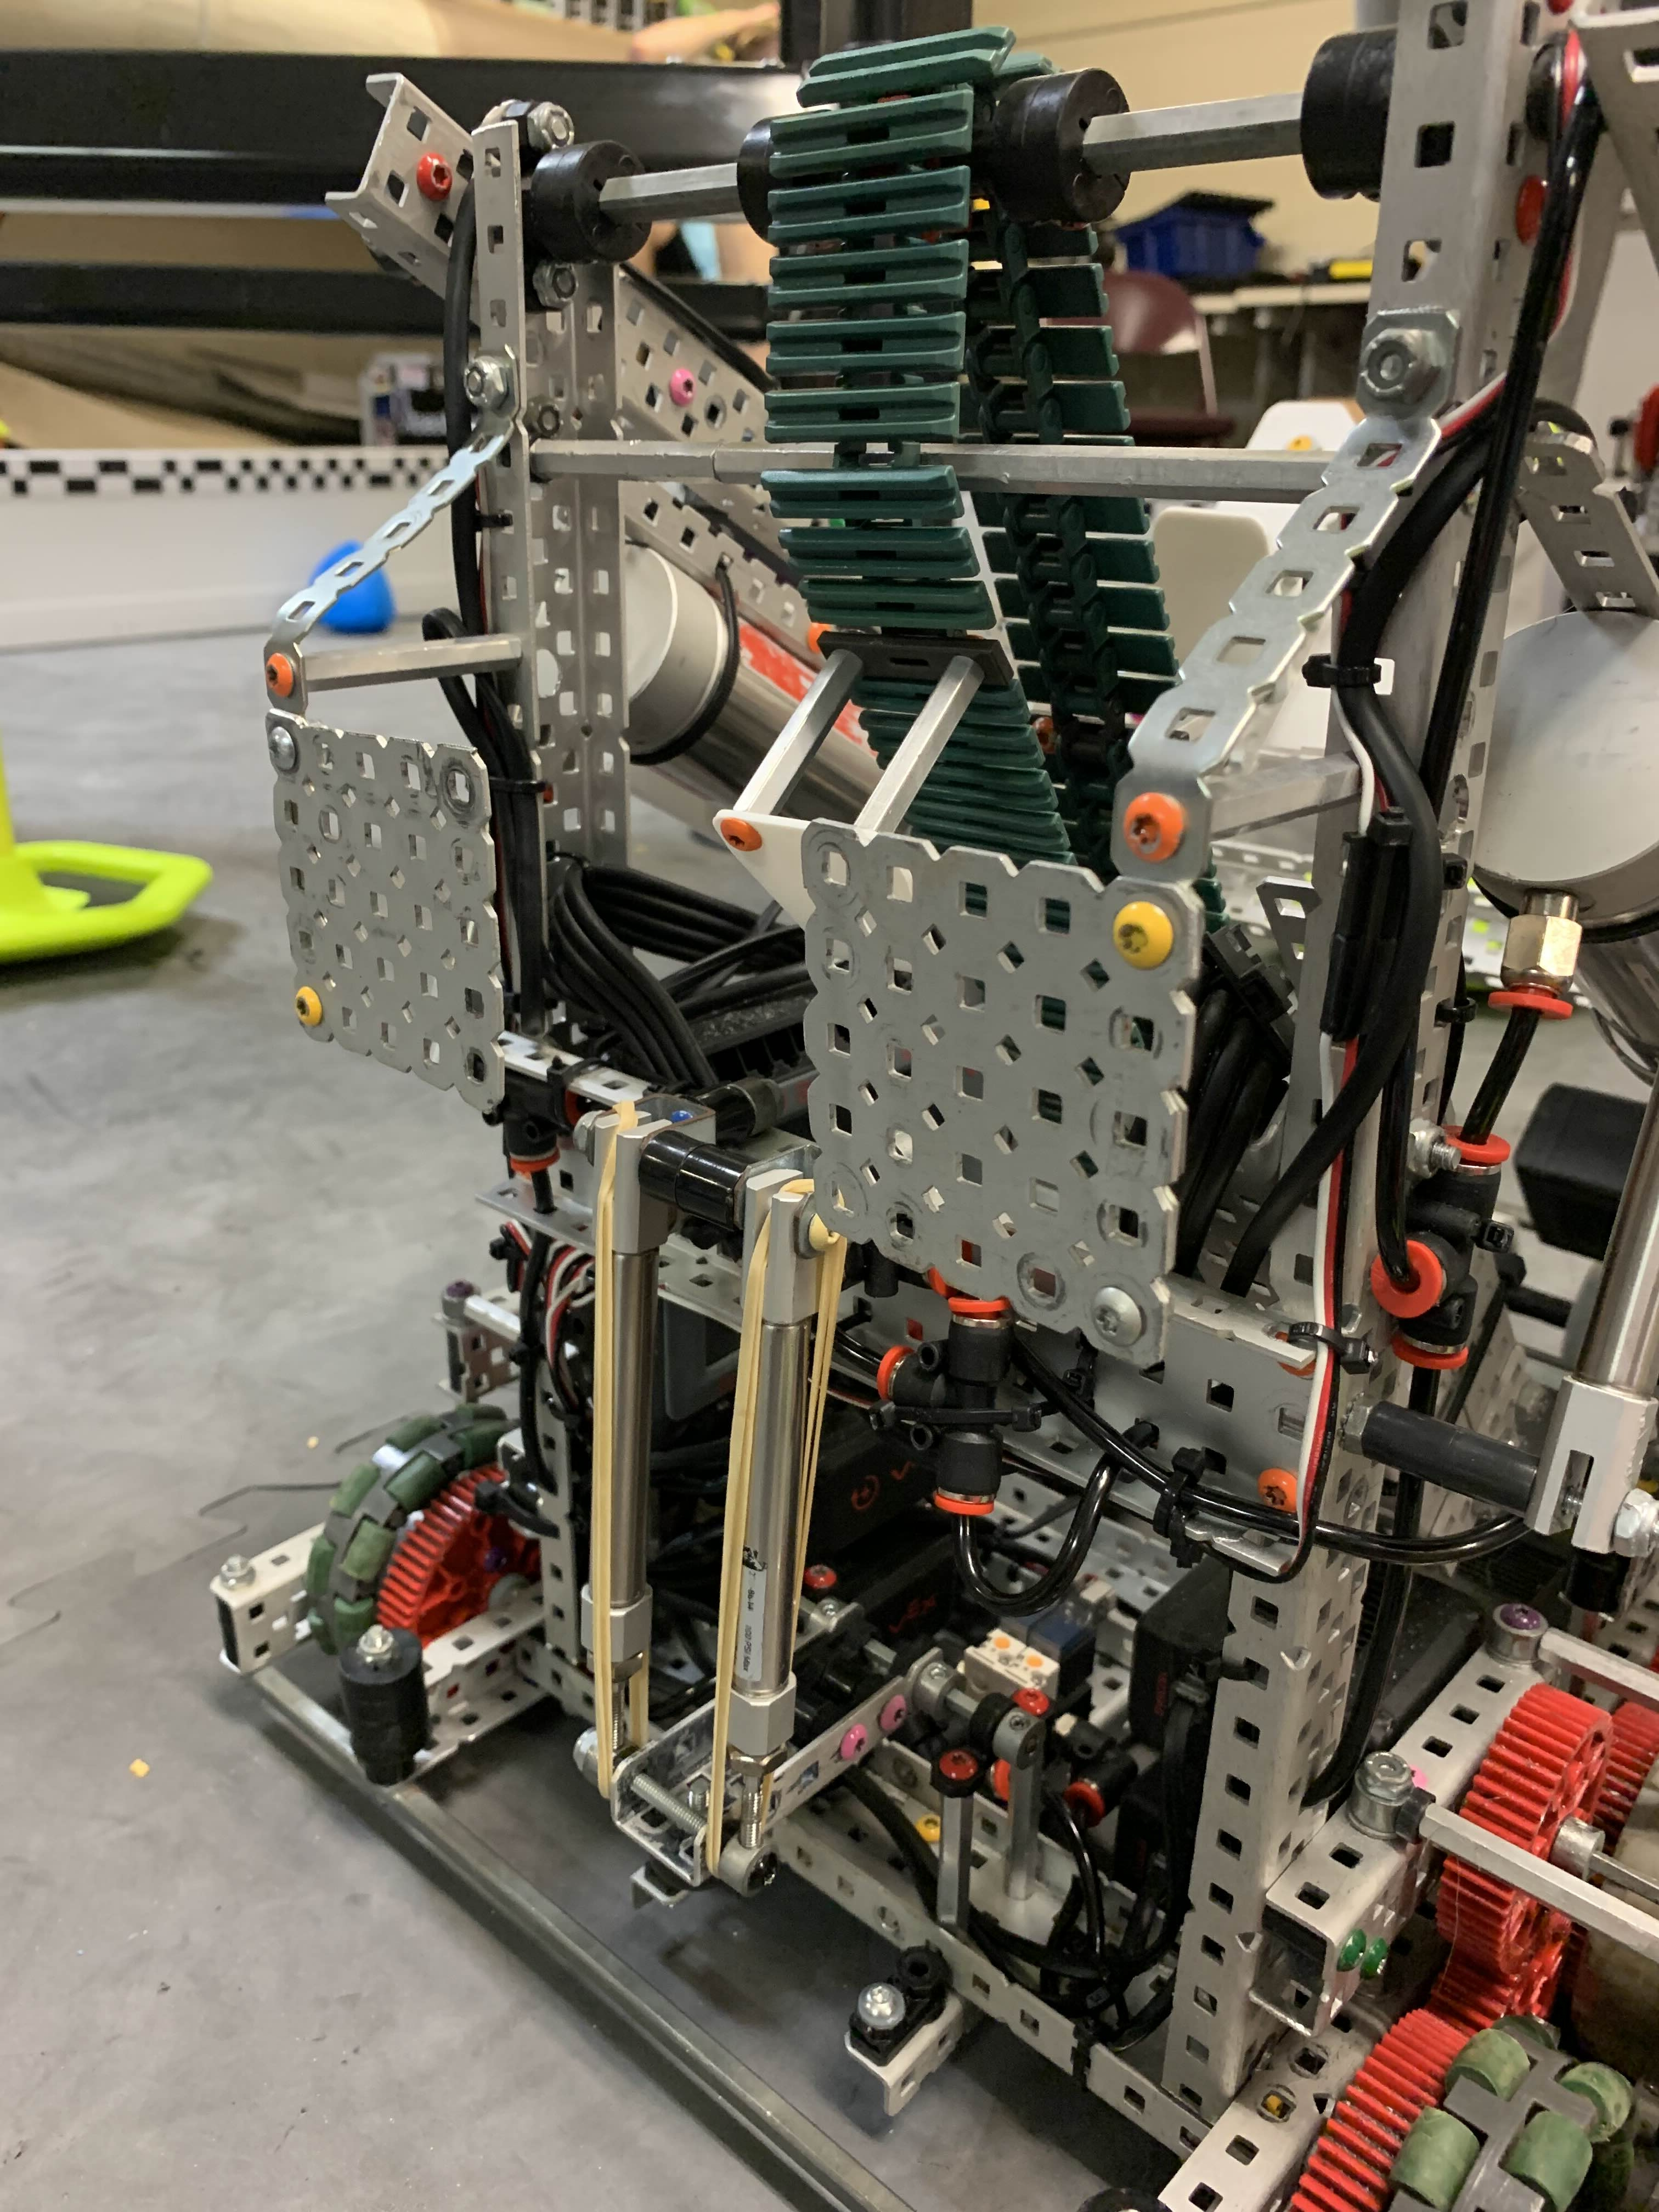
\includegraphics[width=0.5\linewidth]{images/Intake2.jpg}
    \caption{Our intake solution}
    \label{intake2}
\end{figure}
%Add subsections about different building parts 
\test{Test the Solution: Intake V1.1 (July 27th, 2024)}
\chapterauthor{Caleb Bachmeier}
\info{Caleb Bachmeier}{Test the Solution: Intake Redesign}{July 27, 2024}
\section*{Test the Solution}
Testing this solution was another very easy task. We used our clamp to hold down a mobile goal and loaded five rings on the mobile goal, and our solution worked, the intake no longer gets caught on the fifth ring this is shown in \blueref{intake-test}{this picture below.}
\begin{figure}[h!]
    \centering
    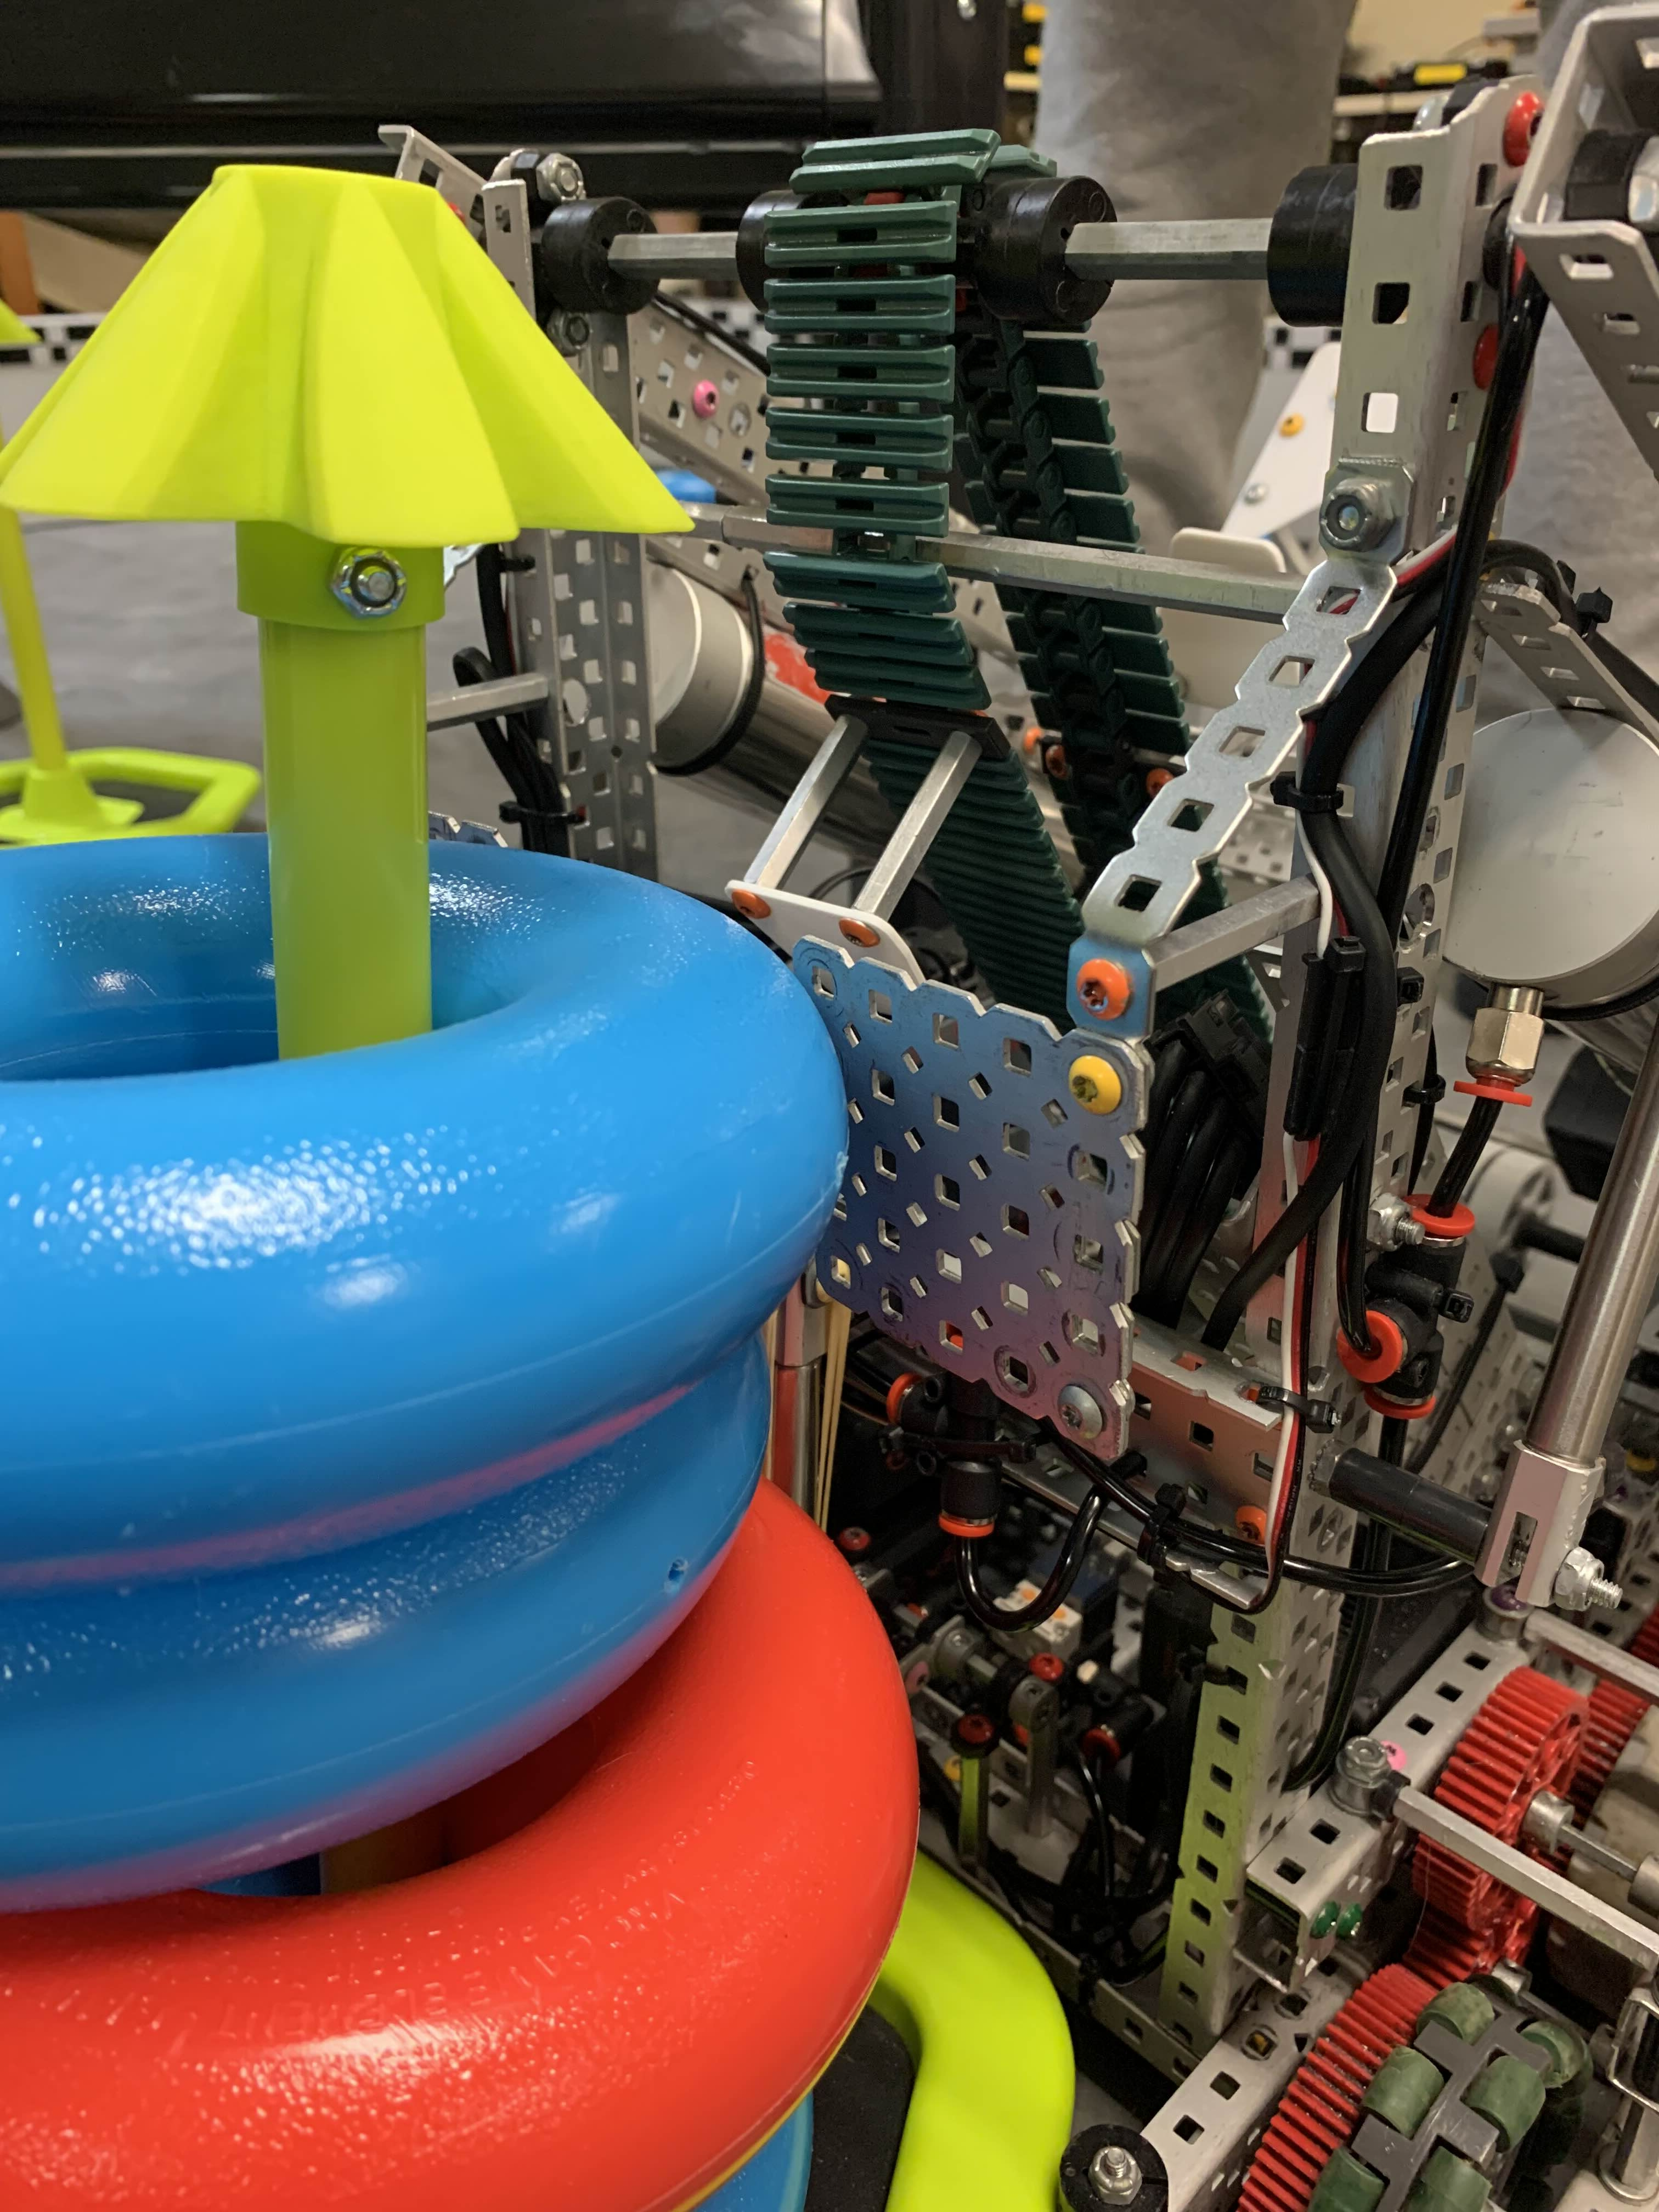
\includegraphics[width=0.5\linewidth]{images/Intake-test.jpg}
    \caption{Our intake solution being tested}
    \label{intake-test}
\end{figure}